\documentclass{article}
\usepackage{graphicx} % Required for inserting images
\usepackage{float}
\usepackage{subcaption}

\title{Linear Regression}
\author{Phan Thanh Binh}

\begin{document}

\maketitle

\section{Implementation}
\begin{itemize}
\item Firstly, we need 3 functions: one for calculate the loss, and each for calculate the derivative for 2 weights $w_0$ and $w_1$.
We implement each function with the 4 input parameters: the 2 weights $w_0$, $w_1$ accompany with the data point $x_i$ and $y_i$.
\item Secondly, for the main gradient descent function, it somewhat has similar inputs as the previous labwork except that it takes in an additional parameter data (i.e. the list of data points). The loss and derivatives are calculated for each data point then average.
\end{itemize}
The full implementation in Python is shown in Figure \ref{fig:impl}.
\begin{figure}[H]
    \centering
    \begin{subfigure}{0.5\linewidth}
        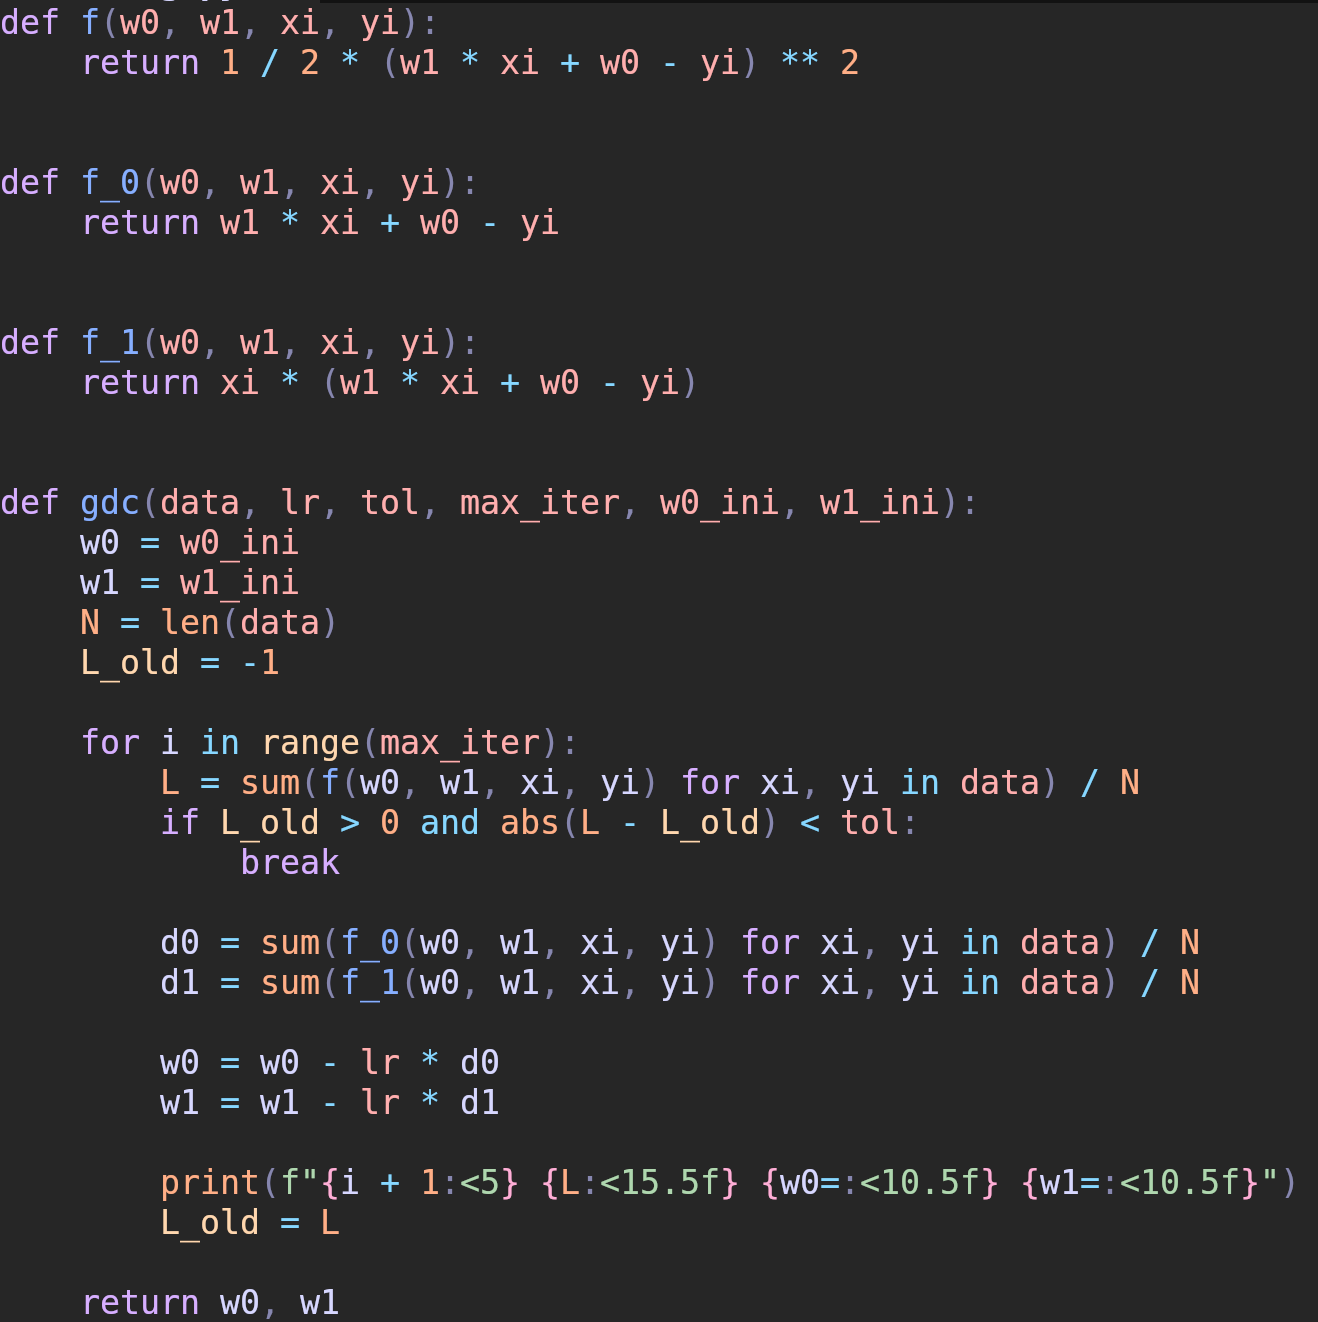
\includegraphics[width=\linewidth]{impl1.png}
    \end{subfigure}
    \begin{subfigure}{0.5\linewidth}
        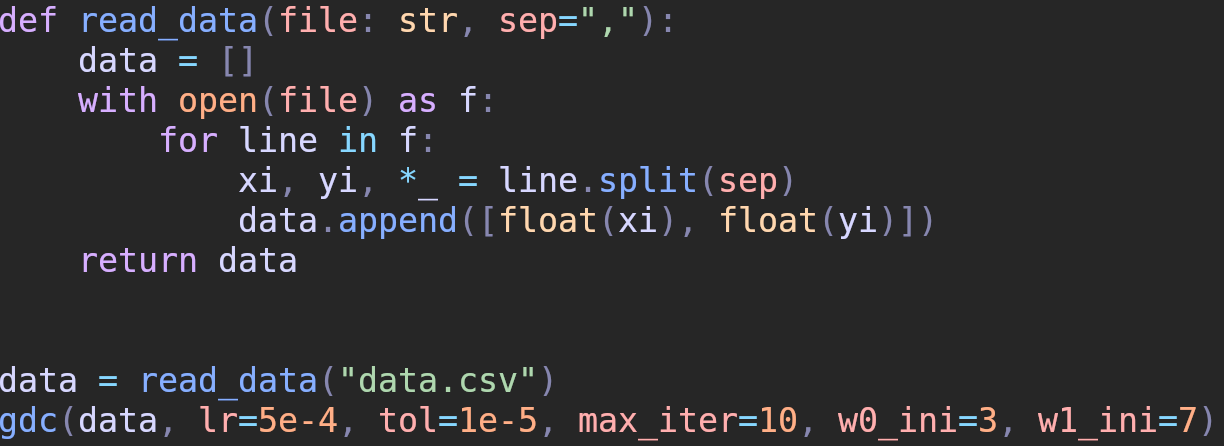
\includegraphics[width=\linewidth]{impl2.png}
    \end{subfigure}
    \caption{Python implementation}
    \label{fig:impl}
\end{figure}

\section{Learning rate effect}
We test the code with different learning rate and plot the loss over the first 10 time steps.
The initial value for $w_0$ and $w_1$ is 7 and 10 respectively.
The effect is clearly shown in the Figure \ref{fig:lrs}, as too big learning rate lead to loss divergence, while too small can lead to slow convergence.
\begin{figure}[H]
\centering
\begin{subfigure}{0.4\textwidth}
    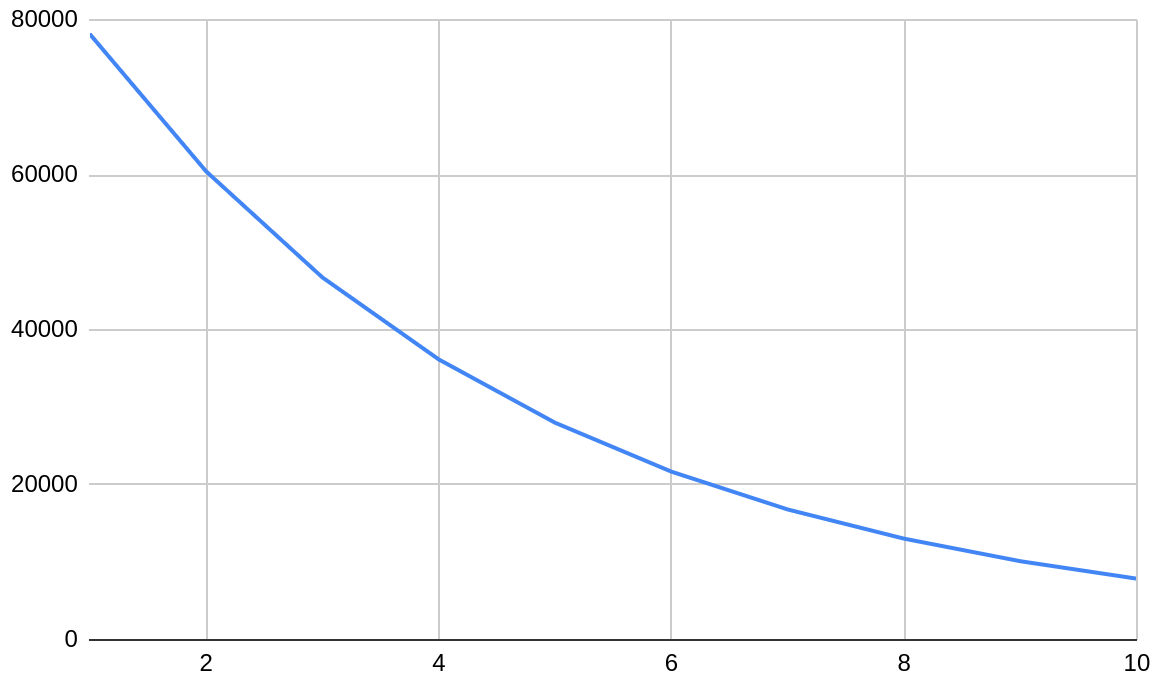
\includegraphics[width=\linewidth]{lr5e5.png}
    \caption{Learning rate = 5e-5}
\end{subfigure}
\begin{subfigure}{0.4\textwidth}
    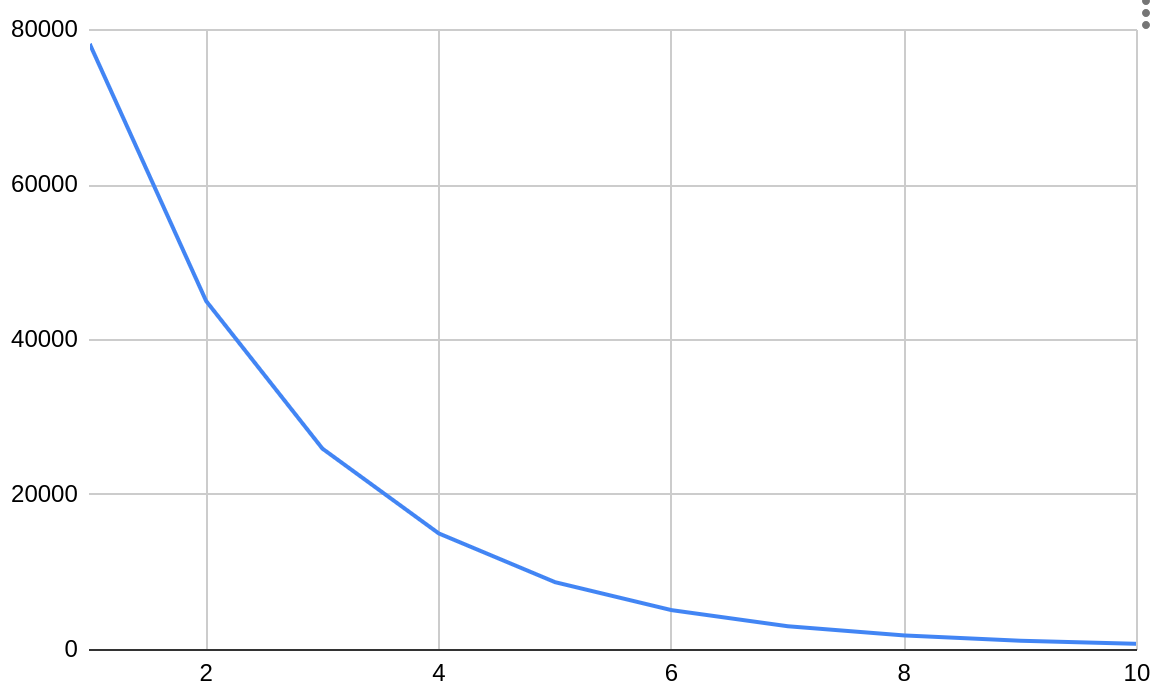
\includegraphics[width=\linewidth]{lr1e4.png}
    \caption{Learning rate = 1e-4}
\end{subfigure}
\begin{subfigure}{0.4\textwidth}
    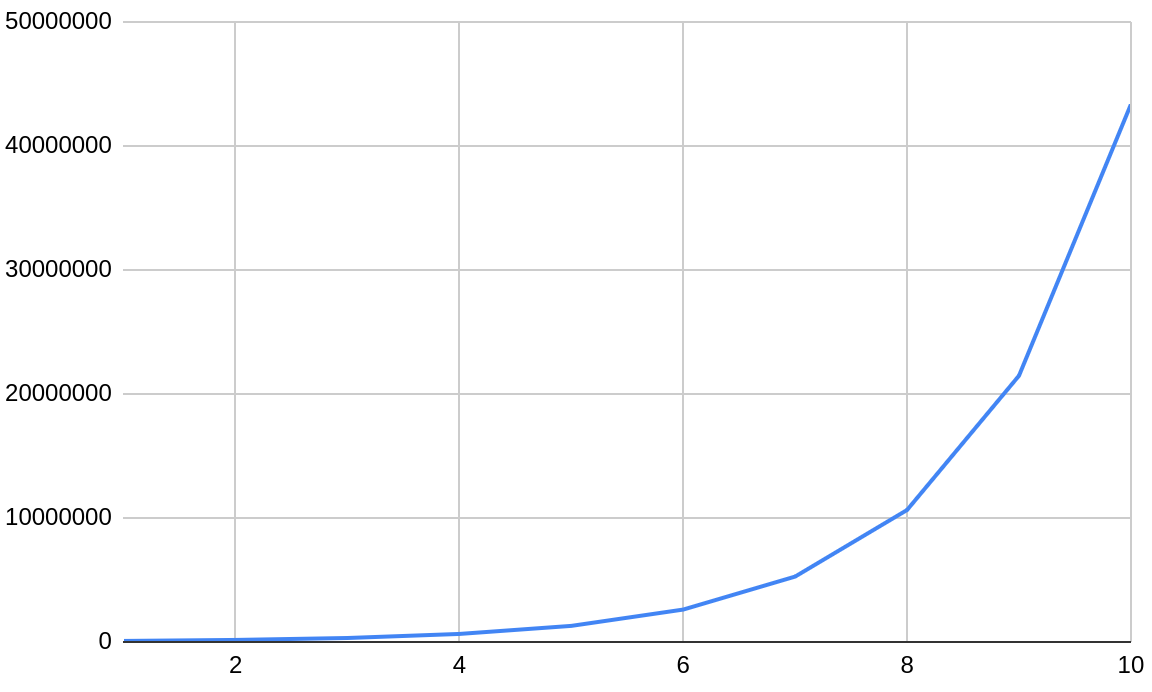
\includegraphics[width=\linewidth]{lr1e3.png}
    \caption{Learning rate = 1e-3}
\end{subfigure}
\caption{Loss values with first 10 time steps with different learning rate}
\label{fig:lrs}
\end{figure}

\end{document}
